% This is LLNCS.DEM the demonstration file of
% the LaTeX macro package from Springer-Verlag
% for Lecture Notes in Computer Science,
% version 2.4 for LaTeX2e as of 16. April 2010
%
\documentclass{llncs}
%
\usepackage{amsmath}
\usepackage{amssymb}
\usepackage{tikz}
\usepackage[linesnumbered,ruled]{algorithm2e}

\newcounter{instr}
\newcommand{\ninstr}{\refstepcounter{instr}\theinstr.}

\begin{document}

\title{Species delimitation}

\titlerunning{Species delimitation}

\author{Tom\'{a}\v{s} Flouri\inst{1} \and Paschalia Kapli\inst{1} \and Sarah Lutteropp\inst{1}}
\authorrunning{Tom\'{a}\v{s} Flouri et al.} % abbreviated author list
\institute{Heidelberg Institute of Theoretical Studies}

\maketitle

\begin{abstract}
An explanation of the Bayesian approach for PTP.\@
\end{abstract}

\section{Bayesian Approach}

In order to obtain support values for every node, we follow a Bayesian Markov-Chain Monte-Carlo (MCMC) approach. We let the user choose whether to start with the maximum likelihood solution found by the heuristic, the null model or a randomly chosen delimitation.

In each MCMC step, we change the current delimitation and recompute its loglikelihood score. After this, we decide whether to keep the change or not according to the hastings ratio. The hastings ratio $r$ is computed as

$$r = \exp(\text{new\_logl} - \text{old\_logl}) * \frac{\text{Number of possible choices for chosen move in old delimitation}}{\text{Number of possible choices for non-chosen move in new delimitation}}$$

\subsection{Allowed Moves}

In order to change a delimitation in the MCMC steps, we randomly select one of two possible moves with equal probability (see Fig.~\ref{fig:moves}).

\begin{figure}[h!]
\centering
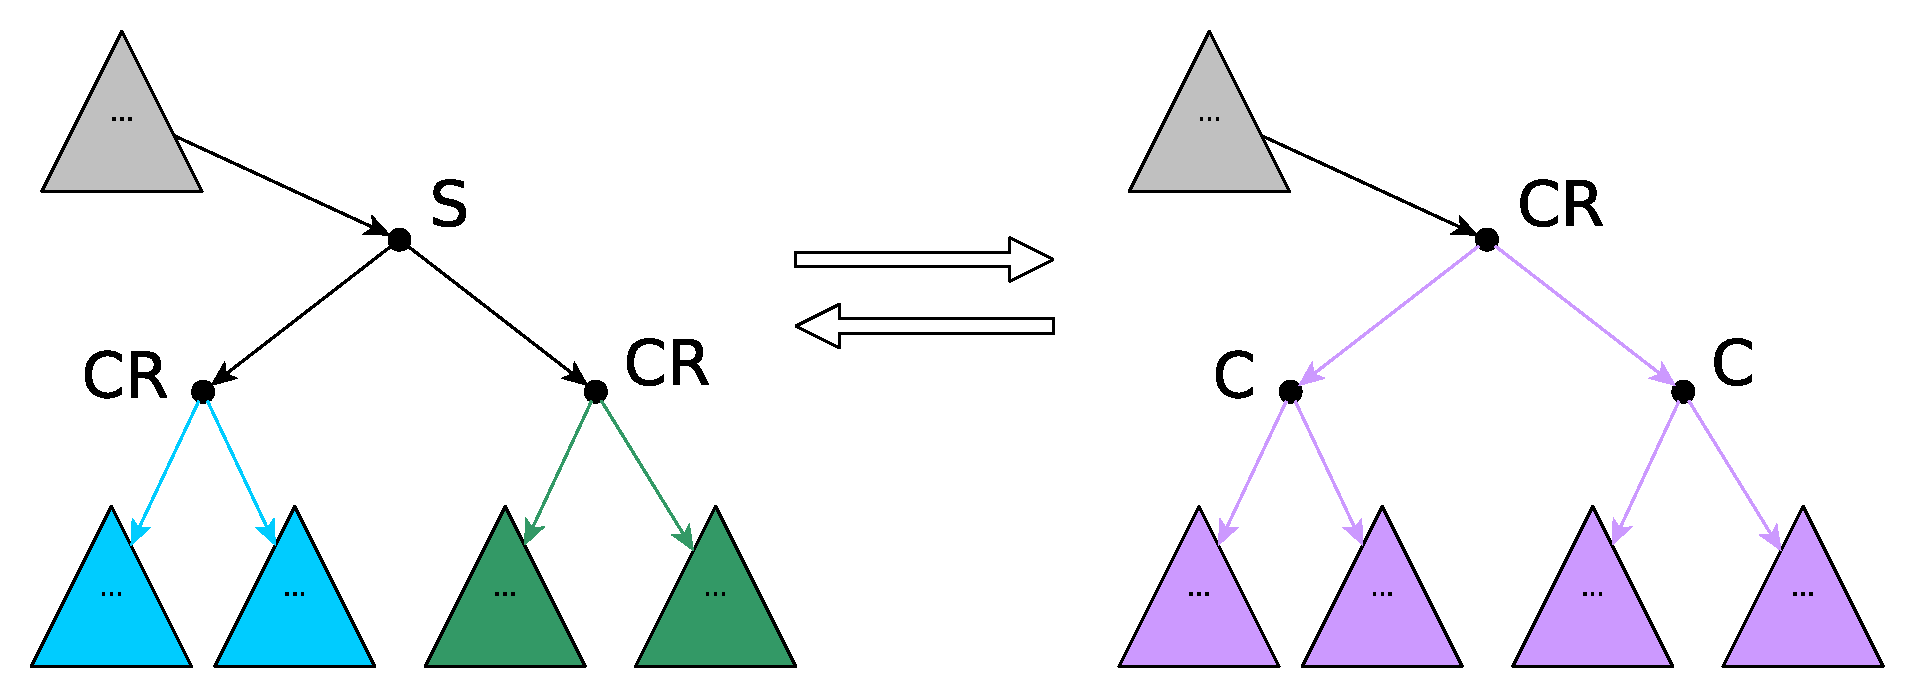
\includegraphics[scale=0.3]{images/moves.pdf}
\caption{Allowed moves in the Bayesian steps. The black edges belong to the speciation part, the colored edges are within species. The node label ``S'' means that a node is a speciation event, whereas the labels ``C'' and ``CR'' mean that a node is a coalescent event. The difference between ``C'' and ``CR'' is that ``CR'' stands for a coalescent root node, i.e. the MRCA of a species.}
\label{fig:moves}
\end{figure}

\subsection{Support Values}
The support value $\text{support}(v)$ of a node $v$ is computed as follows:
$$\text{support}(v) = \frac{\text{Number of MCMC moves without burnin where $v$ was a MRCA}}{\text{Number of MCMC moves without burnin}}$$

\subsection{Pseudocode}

\begin{algorithm}

\underline{function mcmc $(T, min\_br)$}\;
D = getInitialDelimitation($T, min\_br$)\;

\For{$i = 1, \ldots, $ number of runs}{
	p = rand() \textit{//random floating-point number between 0 and 1}\;
	
	\If{$p \leq 0.5$}{
		move = move1\;
	}
	\Else{
		move = move2\;
	}
	D\_new = applyMove(D, move)\;
	
	\If {$i > \text{burnin}$} {
		updateSupportValues(T, D\_new)\;
	}
	r = computeHastingsRatio(D, D\_new, move)\;
	
	q = rand() \textit{//random floating-point number between 0 and 1}\;
	\If{$q \leq r$}{ 
		D = D\_new \textit{//accept move}\;
	}
}

\caption{Markov-Chain Monte-Carlo algorithm for PTP}

\end{algorithm}

\bibliographystyle{splncs03}
\bibliography{delimit}
\end{document}
